\documentclass[letterpaper,12pt]{article}
\usepackage{fullpage}
\usepackage{amsmath,amssymb,amsthm}
\usepackage{enumitem}          % gives custom-labeled enumerations
\usepackage{graphics}
\usepackage{mathabx}
\usepackage{tikz}

\usetikzlibrary{arrows,automata,positioning}
% Draw states as black circles filled with gray.
\tikzstyle{every state}=[fill=black!10]
% Set the size of the double circle around accept states.
\tikzstyle{accepting}=[double=black!10,double distance=2pt,outer sep=1pt+\pgflinewidth]
% No text on start arrows.
\tikzstyle{every initial by arrow}=[initial text=]
% Set bend angle, set the label to appear next to the curve, and set
% the arrow style.
\tikzstyle{every edge}=[draw,bend angle=15,auto,>=stealth']

\setlist[enumerate]{label=\textbf{\alph{*}.},listparindent=1em}

\setlength{\topmargin}{0in}
\setlength{\headheight}{0in}
\setlength{\headsep}{0in}
\setlength{\topskip}{0in}

\newcommand{\Z}{\mathbb{Z}}     % Rich man's black board's font.
\newcommand{\F}{\mathbb{F}}
\newcommand{\R}{\mathbb{R}}

% taken from hs's mary.tex, and tracing back to knuth.
\def\dash---{\kern.16667em---\penalty\exhyphenpenalty\hskip.16667em\relax}

\newcommand{\st}{\;\;\text{s.t.}\;\;}
\newcommand{\rev}{^{\scriptscriptstyle\mathcal{R}}}
\newcommand*\comp{^{\mathcal C}}
% Write alphabet symbols in typewriter font as per Sipser.
\newcommand\s[1]{\ensuremath{\mathtt{#1}}}
\newcommand*\langop{\textsc}

\let\oldsetminus\setminus
\renewcommand*\setminus{\mathbin\oldsetminus}

% Set the exercises number and your name.
\title{Problem Set \#1}
\author{Maxwell Petersen}

% No need to change these 4 lines.
\makeatletter
\newcommand\exercise[1]{\par\vspace{4ex}\normalfont\normalsize\noindent
\textbf{\large Problem #1}\par\nobreak\@afterindentfalse\@afterheading}
\makeatother


\begin{document}
\maketitle

\exercise{1}
Because there is a DFA $M=(Q,\Sigma,\delta,q_0,F)$ that recognizes $A$, building an NFA $N=(Q',\Sigma,\delta',q_0',F')$ that recognizes $A\rev$ proves that $A\rev$ is regular.
The NFA $N=(Q',\Sigma,\delta',q_0',F')$ has $\delta'$ as follows:

\begin{align*}
	\delta'(q_0',\epsilon) &= F\\
	\delta'(q_0',a) &= \emptyset & \forall a \in \Sigma\\
	\delta'(p,a) &= \{q|\delta(q,a) = p\} & \forall q \in Q, a \in \Sigma\\
\end{align*}

\exercise{2}
$\langop{BackwardsAndForwards}(A) = \{w\in A\ |\ \text{$w\in A$ and $w\rev\in A$}\}$ is defined by the closure property of union because the language $A$ and the language $A\rev$ are both regular and union has been proven to keep sets closed.

\exercise{3}
\begin{enumerate}
\item $A\setminus B=\{w\in A\ |\ w\notin B\}$  is a regular and closed language because it is the same thing as $A\cap \thicksim B$ having intersection being proven to keep sets closed if $A$ and $B$ are both regular.
\item $A\mathbin\triangle B=\{w\ |\ \text{either $w\in A$ or $w\in B$ but not both}\}$ is a regular closed set because it has a regular expression ( $A \cup B$)$ \cap \thicksim $($ A \cap B$) with union, intersection, and compliment keeping the set closed.
\end{enumerate}
\cleardoublepage

\exercise{4}
Let there be an alphabet $\Sigma' = \{a' | a \in \Sigma \}$. Let there be homomorphisms un : ($\Sigma \cup \Sigma'$)* $\rightarrow \Sigma$* and rem : ($\Sigma \cup \Sigma'$)* $\rightarrow \Sigma$* such that un($a'$) = $a$ for $a' \in \Sigma'$, un($a$) = $a$ for $a \in \Sigma'$, rem($a'$) = $\epsilon \in \Sigma'$, and rem($a$) = $a$ for $a \in \Sigma$. Let $L_1$ be a language defined as un$^{-1}$($L$) making it regular because languages have been proven to stay closed under inverse homomorphisms, $L_1$ is the subset of strings that may have been marked with an apostrophe. Let there be an $L_2 = L_1 \cap \Sigma'$*$\Sigma$*, $L_2$ is the subset of strings where the first few characters are marked with an apostrophe. $L_2$ Is regular and closed because sets are kept closed and regular with intersection. Because $L_2$ is the same thing as \langop{Suffix} then \langop{Suffix} is seen to be closed and regular as well.

\exercise{5}
$A\obackslash B=\{w\in A\ |\ \text{$w$ does not contain any string in $B$ as a substring}\}$ is a closed set because it has the regular expression of $A \cup (\thicksim B)$ with union and inverse being proven to keep the set closed assuming that $A$ and $B$ are regular.

\exercise{6}
Let there be a DFA $M = (Q,\Sigma,\delta,F)$ which recognizes $A$. Let there also be a NFA $N = (Q', \Gamma,\delta', F')$ which recognizes $f(A)$. The delta transition of $\delta'$ is as follows:
\begin{align*}
	\delta'(q_0',f(\epsilon)) &=  \emptyset\\
	\delta'(q_0',f(a)) &= \delta(q_0,a) & \forall a \in \Gamma\\
	\delta'(p,f(a)) &= \{q|\delta(q,a) = p\} & \forall q \in Q', a \in \Gamma\\
\end{align*}

\exercise{7}
Let there be a DFA $M = (Q,\Sigma,\delta,F)$ which recognizes $A$. Let there also be a NFA $N = (Q', \Gamma*,\delta', F')$ which recognizes $f(A)$. With $f()$ being defined as a homomorphism. The delta transition $\delta'$ is as follows:
\begin{align*}
	\delta'(q_0',f(\epsilon)) &=  \epsilon\\
	\delta'(q_0',f(a)) &= \delta(q_0,f(a)) & \forall a \in \Gamma^*\\
	\delta'(p,f(a)) &= \{q|\delta(q,f(a)) = p\} & \forall q \in Q', a \in \Gamma^*\\
\end{align*}

\exercise{8}
\begin{align*}
A &= \s1  \text{($\s1 \cup \s0$)*}  \s0\\
B &= \s0\text{*}  \s1  \s0\text{*}  \s1  \s0\text{*} \s1   \s0\text{*}\\
C &= \text{($\s1 \cup \s0$)*} \s{0101} \text{($\s1 \cup \s0$)*}\\
D &= \text{($\s1 \cup \s0$)}  \text{($\s1 \cup \s0$)}  \s0  \text{($\s1 \cup \s0$)*}\\
E &= \text{(\s0$$(($\s1 \cup \s0$)}  \text{($\s1 \cup \s0$))*)}  \text{($\s1$($\s1 \cup \s0$)) $$ (($\s1 \cup \s0$) $$ ($\s1 \cup \s0$))*)}\\
F &= \thicksim \text{\s{110}}\\
G &= \text{(\s1 $\cup$ \s0)}  \text{($\s1 \cup \s0$)}  \text{($\s1 \cup \s0$)}  \text{($\s1 \cup \s0$)}  \text{($\s1 \cup \s0$)}\\
H &= \text{($\thicksim$\s{11})} \cup \text{($\thicksim$\s{111})}\\
I &= \text{(\s1}  \text{(\s1 $\cup$ \s0))*} \\
J &= \text{\s0*}  \text{\s1}  \text{\s0*}\\
K &= \text{\s0*}\\
L &= \text{(\s0 $$ \s1* $$ \s0*)*} \cup\text{(\s0* $$ \s1 $$ \s0* $$ \s1 $$ \s0*)}\\
M &= \text{\s1 $\cap \thicksim$ 1}\\
N &= \text{(\s0 $\cap$ \s1)*}\\
\end{align*}

\exercise{9}
Finding the NFA of : $(0\cup 11)^*01(00\cup 1)^*\\$
$\\0:\\$
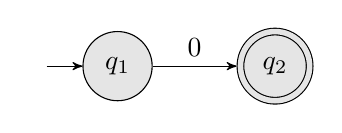
\begin{tikzpicture}[node distance=2cm,initial text=]
  \node[initial,state]        (q1){$q_1$};
  \node[state,accepting]        (q2) [right of=q1]  {$q_2$};

  \path[->] (q1)  edge node {0} (q2);
\end{tikzpicture}
$\\1:\\$
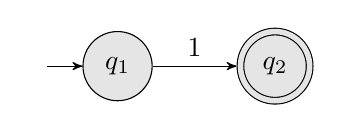
\begin{tikzpicture}[node distance=2cm,initial text=]
  \node[initial,state]        (q1){$q_1$};
  \node[state,accepting]        (q2) [right of=q1]  {$q_2$};

  \path[->] (q1)  edge node {1} (q2);
\end{tikzpicture}
$\\11:\\$
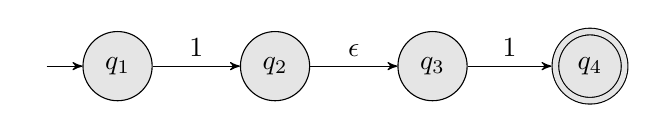
\begin{tikzpicture}[node distance=2cm,initial text=]
  \node[initial,state]        (q1){$q_1$};
  \node[state] 		(q2) [right of=q1]  {$q_2$};
  \node[state]		(q3) [right of=q2]  {$q_3$};
  \node[state,accepting]        (q4) [right of=q3]  {$q_4$};

  \path[->] (q1)  edge node {1} (q2)
  	(q2) edge node {$\epsilon$} (q3)
	(q3) edge node {1}(q4);
\end{tikzpicture}
$\\01:\\$
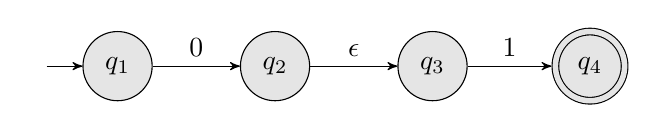
\begin{tikzpicture}[node distance=2cm,initial text=]
  \node[initial,state]        (q1){$q_1$};
  \node[state] 		(q2) [right of=q1]  {$q_2$};
  \node[state]		(q3) [right of=q2]  {$q_3$};
  \node[state,accepting]        (q4) [right of=q3]  {$q_4$};

  \path[->] (q1)  edge node {0} (q2)
  	(q2) edge node {$\epsilon$} (q3)
	(q3) edge node {1}(q4);
\end{tikzpicture}
$\\00:\\$
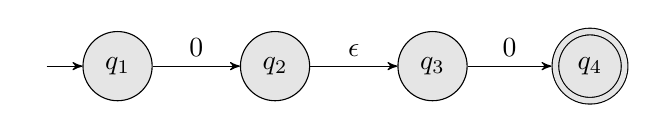
\begin{tikzpicture}[node distance=2cm,initial text=]
  \node[initial,state]        (q1){$q_1$};
  \node[state] 		(q2) [right of=q1]  {$q_2$};
  \node[state]		(q3) [right of=q2]  {$q_3$};
  \node[state,accepting]        (q4) [right of=q3]  {$q_4$};

  \path[->] (q1)  edge node {0} (q2)
  	(q2) edge node {$\epsilon$} (q3)
	(q3) edge node {0}(q4);
\end{tikzpicture}
\cleardoublepage
$\\ 0 \cup 11:\\$
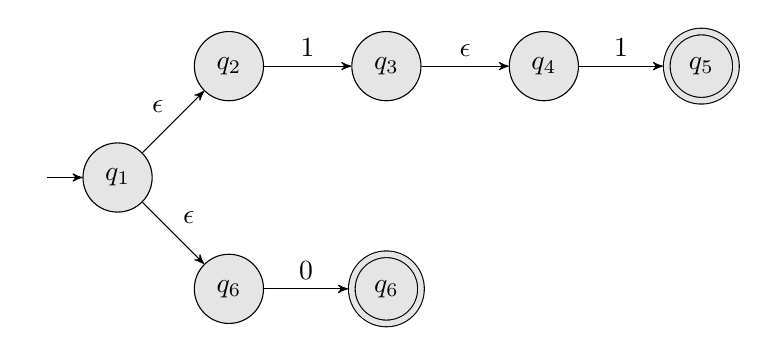
\begin{tikzpicture}[node distance=2cm,initial text=]
  \node[initial,state]        (q1){$q_1$};
  \node[state]		(q2) [above right of=q1]  {$q_2$};
  \node[state] 		(q3) [right of=q2]  {$q_3$};
  \node[state]		(q4) [right of=q3]  {$q_4$};
  \node[state,accepting]        (q5) [right of=q4]  {$q_5$};
  \node[state]        (q6)[below right of=q1] {$q_6$};
  \node[state,accepting]        (q7) [right of=q6]  {$q_6$};

  \path[->] (q1) edge node {$\epsilon$} (q2)
  	        edge node {$\epsilon$} (q6)
  	(q2)  edge node {1} (q3)
  	(q3) edge node {$\epsilon$} (q4)
	(q4) edge node {1}(q5)
	(q6)  edge node {0} (q7);
\end{tikzpicture}
$\\ 00 \cup 1:\\$
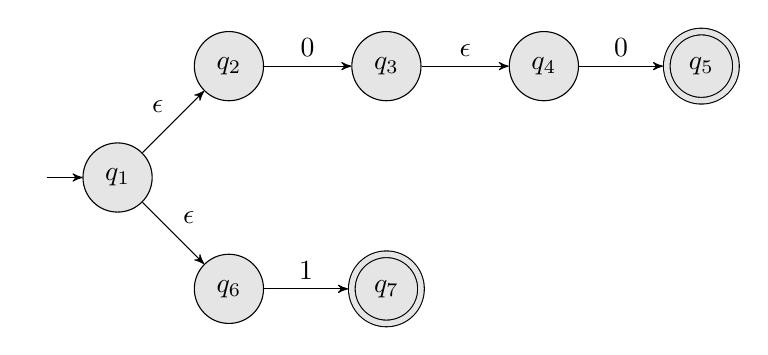
\begin{tikzpicture}[node distance=2cm,initial text=]
  \node[initial,state]        (q1){$q_1$};
  \node[state]		(q2) [above right of=q1]  {$q_2$};
  \node[state] 		(q3) [right of=q2]  {$q_3$};
  \node[state]		(q4) [right of=q3]  {$q_4$};
  \node[state,accepting]        (q5) [right of=q4]  {$q_5$};
  \node[state]        (q6)[below right of=q1] {$q_6$};
  \node[state,accepting]        (q7) [right of=q6]  {$q_7$};

  \path[->] (q1) edge node {$\epsilon$} (q2)
  	        edge node {$\epsilon$} (q6)
  	(q2)  edge node {0} (q3)
  	(q3) edge node {$\epsilon$} (q4)
	(q4) edge node {0}(q5)
	(q6)  edge node {1} (q7);
\end{tikzpicture}
$\\ (0 \cup 11)^*:\\$
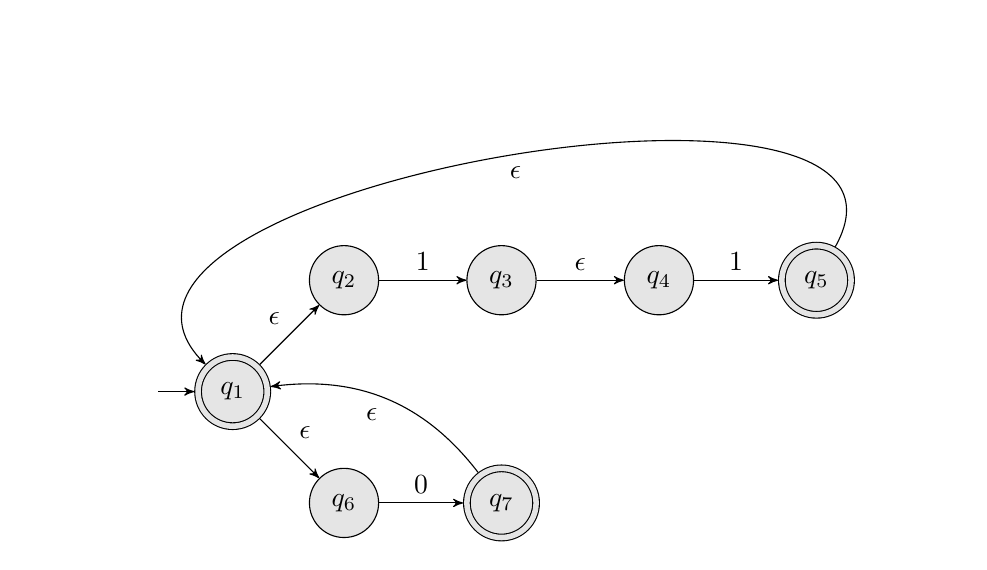
\begin{tikzpicture}[node distance=2cm,initial text=]
  \node[initial,state,accepting]        (q1){$q_1$};
  \node[state]		(q2) [above right of=q1]  {$q_2$};
  \node[state] 		(q3) [right of=q2]  {$q_3$};
  \node[state]		(q4) [right of=q3]  {$q_4$};
  \node[state,accepting]        (q5) [right of=q4]  {$q_5$};
  \node[state]        (q6)[below right of=q1] {$q_6$};
  \node[state,accepting]        (q7) [right of=q6]  {$q_7$};

  \path[->] (q1) edge node {$\epsilon$} (q2)
  	        edge node {$\epsilon$} (q6)
  	(q2)  edge node {1} (q3)
  	(q3) edge node {$\epsilon$} (q4)
	(q4) edge node {1}(q5)
	(q6) edge node {0} (q7)
	(q5) [out=225 in=0] edge node {$\epsilon$} (q1)
	(q7) [bend right] edge node {$\epsilon$} (q1);
\end{tikzpicture}
\cleardoublepage
$\\ (00 \cup 1)^*:\\$
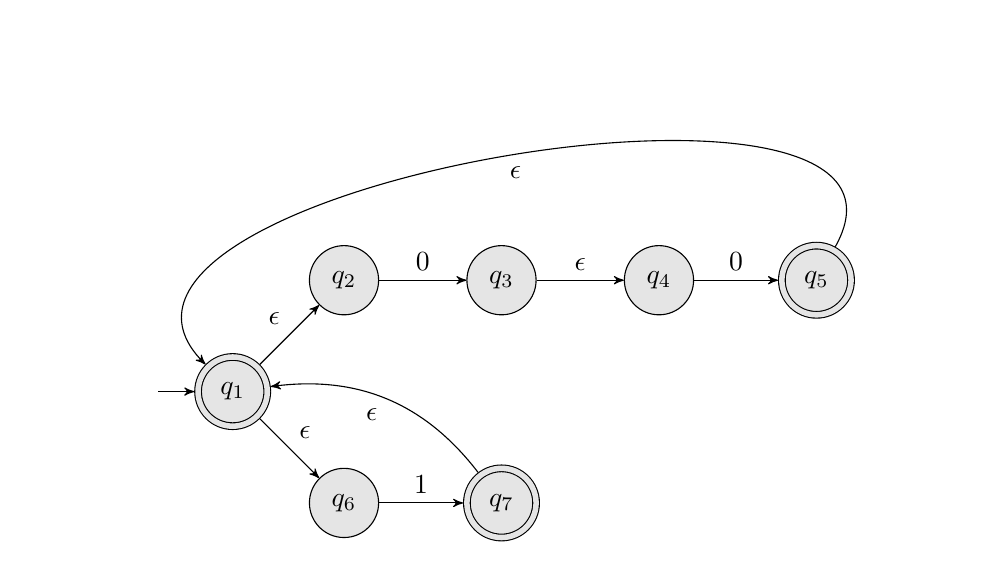
\begin{tikzpicture}[node distance=2cm,initial text=]
  \node[initial,state, accepting]        (q1){$q_1$};
  \node[state]		(q2) [above right of=q1]  {$q_2$};
  \node[state] 		(q3) [right of=q2]  {$q_3$};
  \node[state]		(q4) [right of=q3]  {$q_4$};
  \node[state,accepting]        (q5) [right of=q4]  {$q_5$};
  \node[state]        (q6)[below right of=q1] {$q_6$};
  \node[state,accepting]        (q7) [right of=q6]  {$q_7$};

  \path[->] (q1) edge node {$\epsilon$} (q2)
  	        edge node {$\epsilon$} (q6)
  	(q2)  edge node {0} (q3)
  	(q3) edge node {$\epsilon$} (q4)
	(q4) edge node {0}(q5)
	(q6) edge node {1} (q7)
	(q5) [out=225 in=0] edge node {$\epsilon$} (q1)
	(q7) [bend right] edge node {$\epsilon$} (q1);
\end{tikzpicture}
$\\ (0\cup 11)^*01 \\$
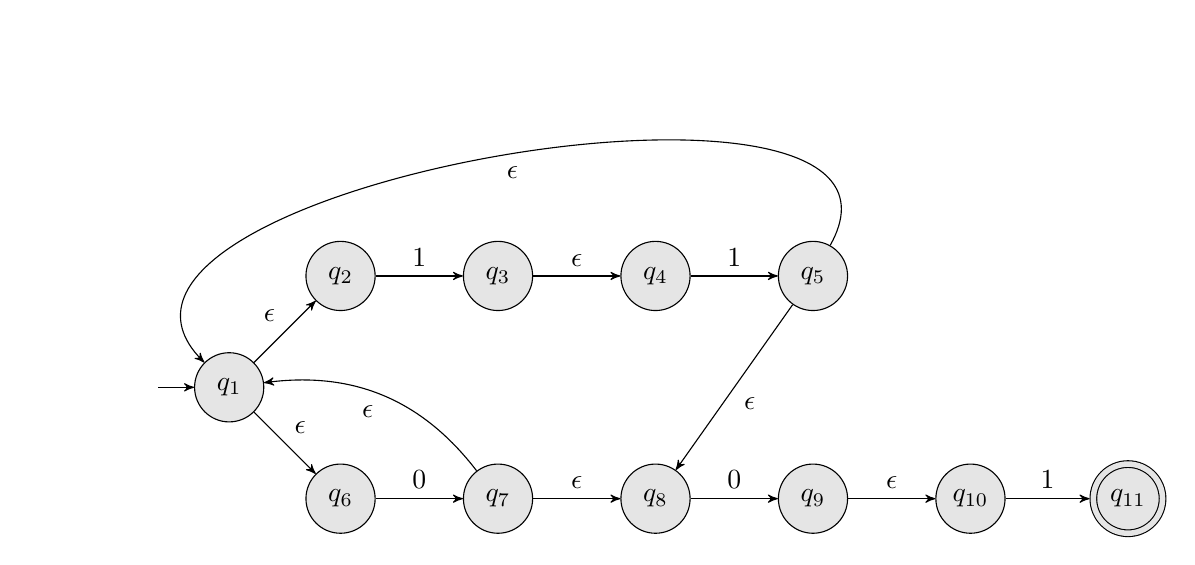
\begin{tikzpicture}[node distance=2cm,initial text=]
  \node[initial,state]        (q1){$q_1$};
  \node[state]		(q2) [above right of=q1]  {$q_2$};
  \node[state] 		(q3) [right of=q2]  {$q_3$};
  \node[state]		(q4) [right of=q3]  {$q_4$};
  \node[state]		(q5) [right of=q4]  {$q_5$};
  \node[state]		(q6)[below right of=q1] {$q_6$};
  \node[state]		(q7) [right of=q6]  {$q_7$};
  \node[state]		(q8) [right of=q7]  {$q_8$};
  \node[state]		(q9) [right of=q8]  {$q_9$};
  \node[state]		(q10) [right of=q9]  {$q_{10}$};
  \node[state,accepting]        (q11) [right of=q10]  {$q_{11}$};

  \path[->] (q1) edge node {$\epsilon$} (q2)
  	        edge node {$\epsilon$} (q6)
  	(q2)  edge node {1} (q3)
  	(q3) edge node {$\epsilon$} (q4)
	(q4) edge node {1}(q5)
	(q6) edge node {0} (q7)
	(q7) edge node {$\epsilon$} (q8)
	(q5) edge node {$\epsilon$} (q8)
	(q8) edge node {0} (q9)
	(q9) edge node {$\epsilon$}(q10)
	(q10) edge node {1}(q11)
	(q5) [out=225 in=0] edge node {$\epsilon$} (q1)
	(q7) [bend right] edge node {$\epsilon$} (q1);
\end{tikzpicture}
\cleardoublepage
$\\(0\cup 11)^*01(00\cup 1)^*\\$
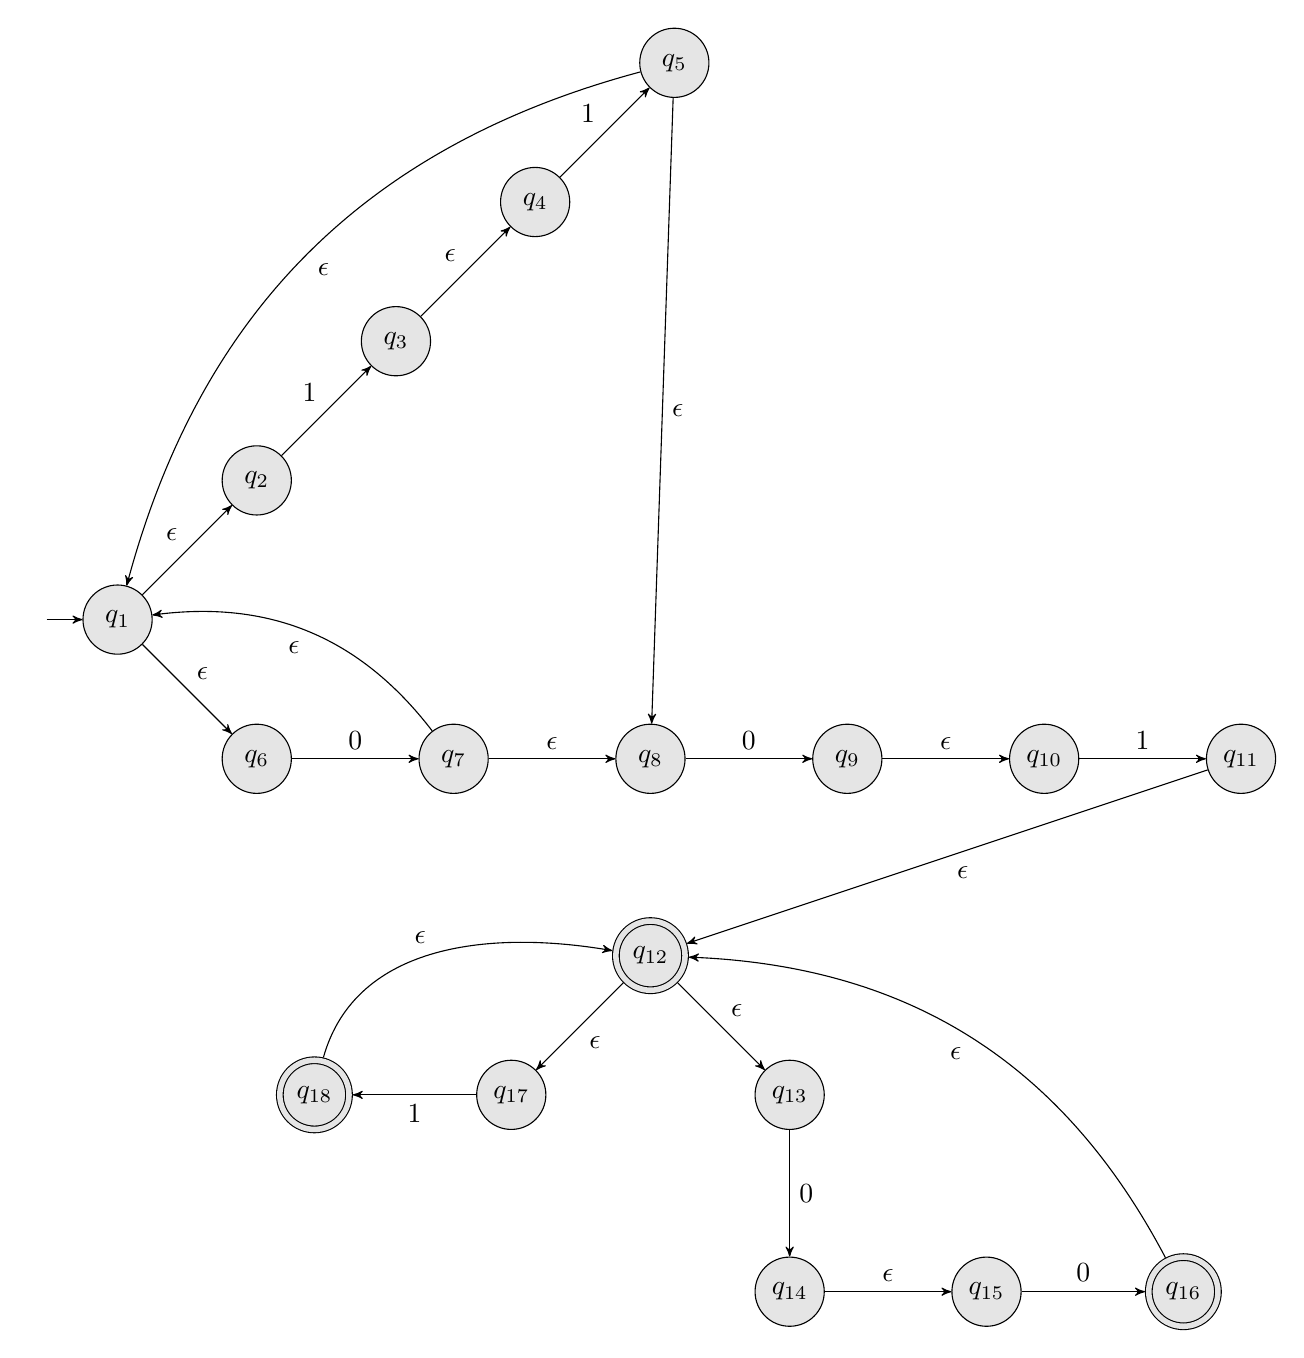
\begin{tikzpicture}[node distance=2.5cm,initial text=]
  \node[initial,state]        (q1){$q_1$};
  \node[state]		(q2) [above right of=q1]  {$q_2$};
  \node[state] 		(q3) [above right of=q2]  {$q_3$};
  \node[state]		(q4) [above right of=q3]  {$q_4$};
  \node[state]		(q5) [above right of=q4]  {$q_5$};
  \node[state]		(q6)[below right of=q1] {$q_6$};
  \node[state]		(q7) [right of=q6]  {$q_7$};
  \node[state]		(q8) [right of=q7]  {$q_8$};
  \node[state]		(q9) [right of=q8]  {$q_9$};
  \node[state]		(q10) [right of=q9]  {$q_{10}$};
  \node[state]        	(q11) [right of=q10]  {$q_{11}$};
  \node[state, accepting]        	(q12) [below of=q8]{$q_{12}$};
  \node[state]		(q13) [below right of=q12]  {$q_{13}$};
  \node[state] 		(q14) [below of=q13]  {$q_{14}$};
  \node[state]		(q15) [right of=q14]  {$q_{15}$};
  \node[state,accepting]        (q16) [right of=q15]  {$q_{16}$};
  \node[state]        (q17)[below left of=q12] {$q_{17}$};
  \node[state,accepting]        (q18) [left of=q17]  {$q_{18}$};

  \path[->] (q1) edge node {$\epsilon$} (q2)
  	        edge node {$\epsilon$} (q6)
  	(q2)  edge node {1} (q3)
  	(q3) edge node {$\epsilon$} (q4)
	(q4) edge node {1}(q5)
	(q6) edge node {0} (q7)
	(q7) edge node {$\epsilon$} (q8)
	(q5) edge node {$\epsilon$} (q8)
	(q8) edge node {0} (q9)
	(q9) edge node {$\epsilon$} (q10)
	(q10) edge node {1} (q11)
	(q11) edge node {$\epsilon$} (q12)
	(q12) edge node {$\epsilon$} (q13)
  	        edge node {$\epsilon$} (q17)
  	(q13)  edge node {0} (q14)
  	(q14) edge node {$\epsilon$} (q15)
	(q15) edge node {0}(q16)
	(q17) edge node {1} (q18)
	(q16) [bend right] edge node {$\epsilon$} (q12)
	(q18) [bend left, out= 200 in=80] edge node {$\epsilon$} (q12)
	(q5) [bend right] edge node {$\epsilon$} (q1)
	(q7) [bend right] edge node {$\epsilon$} (q1);
\end{tikzpicture}

\end{document}
